\begin{figure}[ht!]
  \centering
  \caption{Overview of countries} \label{fig:Map}
  \begin{subfigure}[b]{\textwidth}
  \centering
    \caption{Country clusters} \label{fig:Map_1}
  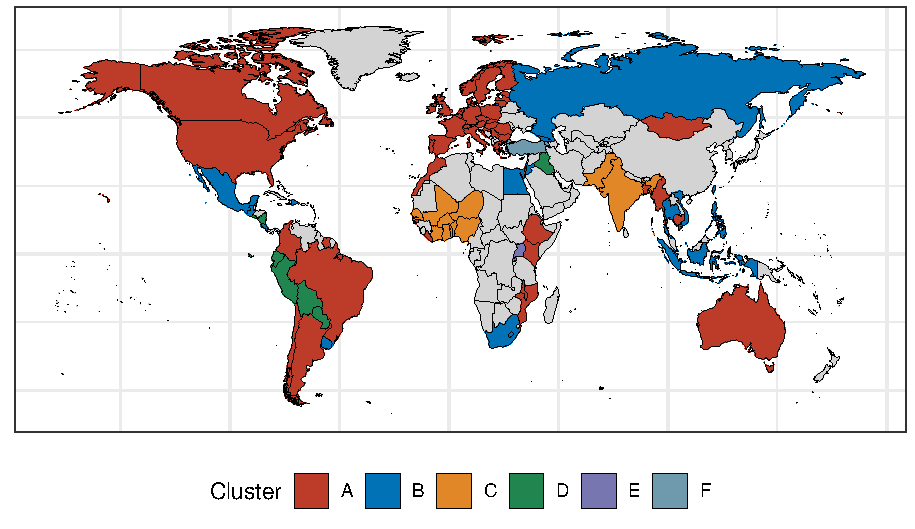
\includegraphics{1_Figures/Figures_Appendix/Figure_Maps_1.pdf}
  \begin{subcaption2}
    This figure shows a map of all countries in our sample. Colour refers to each country's cluster. See also table \ref{tab:A10}.
  \end{subcaption2}
  \end{subfigure}
\end{figure}

\begin{figure}[ht!]\ContinuedFloat
   \begin{subfigure}[b]{\textwidth}
  \centering
      \caption{Goodness of fit (R\textsuperscript{2}) for each country} \label{fig:Map_2}
  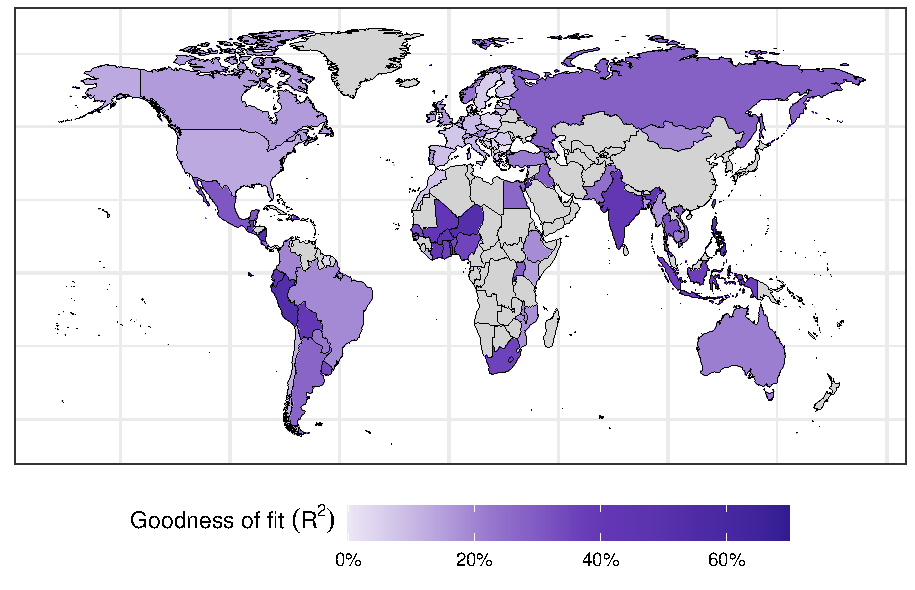
\includegraphics{1_Figures/Figures_Appendix/Figure_Maps_2.pdf}
  \begin{subcaption2}
    This figure shows a map of all countries in our sample. Colour refers to the goodness of fit (R\textsuperscript{2}) for boosted regression tree models, fitted for each country.
  \end{subcaption2}
\end{subfigure}
\end{figure}

\clearpage

\begin{figure}[ht!]\ContinuedFloat
   \begin{subfigure}[b]{\textwidth}
  \centering
    \caption{Most important feature for each country} \label{fig:Map_3}
  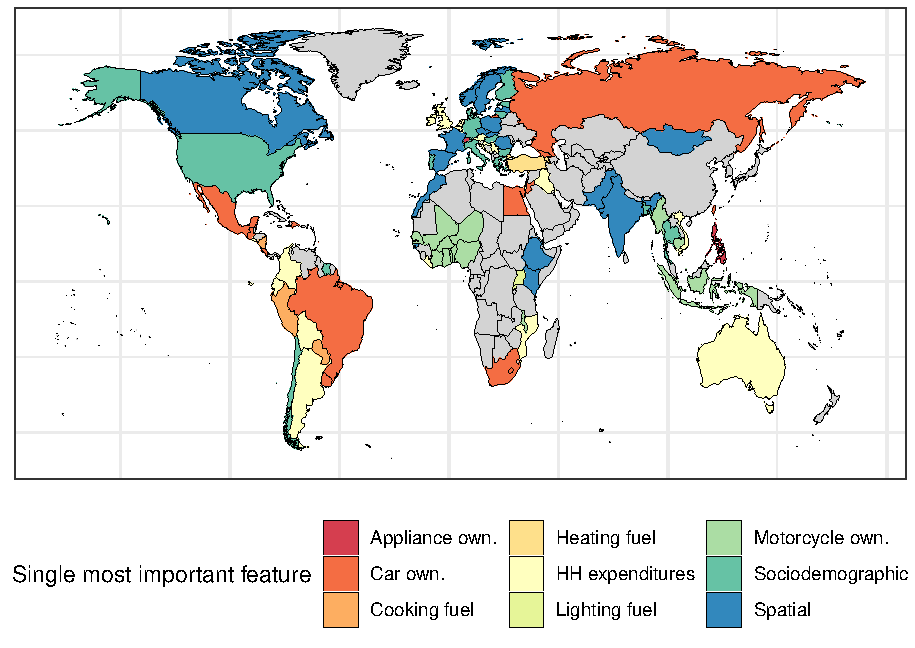
\includegraphics{1_Figures/Figures_Appendix/Figure_Maps_3.pdf}
  \begin{subcaption2}
    This figure shows a map of all countries in our sample. Colour refers to the most important feature in boosted regression tree models, fitted for each country.
  \end{subcaption2}
\end{subfigure}
\end{figure}